We have seen that even problems with multiple dimensions of
flexibility can be solved in polynomial time. We presented dynamic programming-based solution for
jointly optimization of flexible node placement, assigning multiple
chunks to the same VM, communication among VMs, even under capacity
constraints ($\FP+\MA+\CC+\BW$). We were able to produce solution for optimizing replica selection,
multiple assignment, VM communication, under capacity constraints in
scenario where VMs are already spawned in certain nodes ($\RS+\MA+\CC+\BW$).



This section now points out fundamental
limitations in terms of computational tractability. In particular, we
will show that problems become NP-hard if multiple replicas have to be
assigned to a node ($\FP+\RS+\MA$ is proved NP-hard in
Section~\ref{ssec:fprsma}) or if inter-connects have to be established
($\FP+\RS+\CC$ is proved NP-hard in Section~\ref{ssec:fprscc}); both
results hold even in uncapacitated networks, and even in trees
consisting of two levels only (e.g., in a
datacenter \emph{pod}). Hardness of those problem variants will result
in hardness of 4 other variants -- see generalization graph below.


\begin{figure}[htbp]
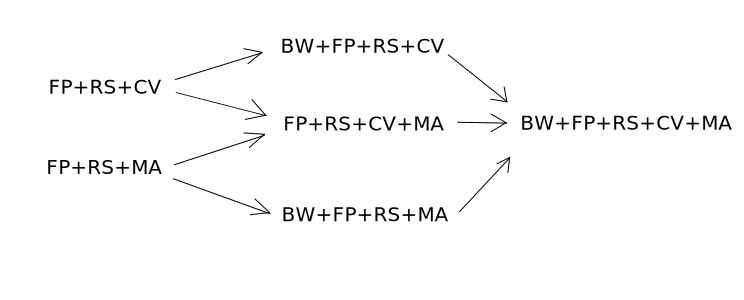
\includegraphics[width = \columnwidth]{figs/np-hierarchy}
\end{figure}



\subsection{Introduction to 3D Perfect Matching}

We start by introducing the NP-complete problem of 3D Perfect Matching
that will serve as problem we reduce from in both proofs. This problem
can be seen as a generalization of bipartite matchings to 3-uniform
hypergraphs, henceforth called $\TDM$.~\cite{3dmatch}

$\TDM$ is defined as follows. We are given three finite and disjoint
sets $X$, $Y$, and $Z$ of cardinality $k$, as well as a subset of triples $T\subset
X \times Y \times Z$.  Set $M \subseteq T$ is a 3-dimensional matching
if and only if, for any two distinct triples $(x_1, y_1, z_1) \in M$
and $(x_2, y_2, z_2) \in M$, it holds that $x_1\neq x_2$, $y_1\neq
y_2$, and $z_1\neq z_2$. Our goal is to decide if we can construct
such $M \subseteq T$ that is perfect, which means that it covers all
elements of $X \times Y \times Z$.

TODO: cite Karp on result of NP-completeness
TODO: image like this: \url{https://upload.wikimedia.org/wikipedia/commons/thumb/5/50/3-dimensional-matching.svg/240px-3-dimensional-matching.svg.png}

\subsection{Multi-Assignments are hard ($\FP+\RS+\MA$)}\label{ssec:fprsma}

Here we will present high-level ideas about encoding $\TDM$ as
 $\FP+\RS+\MA$ instance:

 \begin{itemize} \item For every element of universe $X\cup Y\cup
 Z$, we create chunk type. Processing every chunk corresponds to
 covering whole universe.

 \item We will encode each tripple as $3$ leaves that are close to
 eachother. We place chunk replicas that correspond to elements of the
 tripple.

 \item Placement of VMs will correspond to choice of tripples. No
 matter in which leaf of the gadget the VM will spawn, we will take
 that tripple to solution. VM will process the chunk that it sits on
 top of, as well as chunks in other two leaves of the same gadget.
 
\item We will set threshold cost in such way that no VM process
any chunk outside of the gadget that VM sits in.
\end{itemize}

\textbf{Construction.}
Given an instance $I$ of $\TDM$, we construct an instance $I'$ of
$\FP+\RS+\MA$ as follows:
\begin{itemize}
\item (tree construction) We create a tree consisiting of root vertex,
and for each tripple we create a gadget that we attach as direct child
of the root. We construct a height-2 gadget
as follows. For each tripple $T_i$ we construct a gadget
consisting of an inner node (a router) and three leaves.
\item (chunks and chunk replicas) For each element in $X$, $Y$ and $Z$ we create chunk type
($3 \cdot k$ in total). Every gadget
contains three chunk replicas, corresponding to the elements of $T_i$.
\item (other properties) We set number of VMs to spawn to $k$; we set
$\CostTrans=1$; we set number of slots in each VM to $m=3$; we set
$\Thr=2 \cdot 2 \cdot k$
\end{itemize}

FIXME: The construction is illustrated in Figure~\ref{fig:fprsma}.

\textbf{Correctness.}
We can now show the computational hardness.
\begin{theorem}
$\FP+\RS+\MA$ is NP-hard.
\end{theorem}
\begin{proof}
Let $I$ be an instance of $\TDM$ and let $I'$ be an instance of
$\FP+\RS+\MA$ constructed as described above.
We prove that $I'$ has solution of cost $\leq \Thr$ if ($\Rightarrow$) and only if
($\Leftarrow$)
$I$ has a matching of size $k$.

($\Rightarrow$) Let us take a solution to $\TDM$. We spawn VM in every
gadget that corresponds to chosen triples. We match every chunk in a
gadget to machine in this gadget (only for chosen ones). Solution has
cost exactly $\Thr$. As every element of universe was covered, every
chunk type is processed.

($\Leftarrow$) Let's take solution to $VC$ instance of cost $\leq \Thr$. We
chose triples that correspond to gadgets where there were VMs. Everything
was processed, therefore every element of X,Y and Z is matched. Each
VM processed chunks that correspond to the tripple, otherwise the
solution would have cost larger than $\Thr$, because of 
transportation cost over longer distance.
\end{proof}


\subsection{Inter-connects are hard ($\FP+\RS+\CC$)}\label{ssec:fprscc}


Next, we prove that the joint optimization of node placement and replica selection
is NP-hard if an inter-connect has to be established between virtual machines.
In our terminology, this is the $\FP+\RS+\CC$ problem.

\textbf{Construction.}
Concretely, let $I$ be an instance of $\TDM$. We will create an instance $I'$
for $\FP+\RS+\CC$ as follows:
\begin{itemize}
\item We will construct the same tree as in previous reduction with
chunk replicas placed in the same way.
\item We set the access cost $\CostTrans$ to a chunk replica to a high value $W$. This will force
nodes to be collocated with the replica.
(For now, we can assume that $W=\infty$; a lower and sufficient bound will be given
in the appendix.)
\item The communication cost in the inter-connect is set to $\CostCom = 1$.
\item The number of nodes (virtual machines) is $\Vms = 3 \cdot k$.
\item We use a threshold $\Thr =  6 \cdot k + 3 \cdot 3 \cdot 2 \cdot
(k - 1) \cdot k$.
\end{itemize}

FIXME: The construction is illustrated in Figure~\ref{fig:fprscc}.

\textbf{Proof of correctness.}
Intuitively, in order to minimize embedding costs,
nodes should be placed on near-by replicas. We use the following
helper lemma.
\begin{lemma}\label{lemma:helper}
In every valid solution $\Sol$ of $I'$ of cost $\leq \Thr$, each gadget
falls in one of two categories:
$k$ gadgets have exactly
$3$ nodes, and $n-k$ gadgets remain empty.
\end{lemma}
\begin{proof}
Since $W=\infty$, nodes will always be placed
directly on chunks (the access network cost is zero).
Moreover, since
$\Sol$ is valid, $3 \cdot k$ nodes are mapped
directly to the different chunk locations.
Now, consider any pair of nodes communicating over the
inter-connect; due to our construction, the communication cost
for each such pair is either
2 hops (if they belong to the same gadget) or 4 hops (if they belong
to different gadgets).
The lemma then follows from the observation that $\Thr$
is chosen such that it is never possible to distribute nodes
among more than $k$ gadgets.
\end{proof}

\begin{theorem}
$\FP+\RS+\CC$ is NP-hard.
\end{theorem}
\begin{proof}
Let $I$ be an instance of $\TDM$ and let $I'$ be an instance of
$\FP+\RS+\CC$ constructed as described above.
We prove that $I'$ has solution of cost $\leq \Thr$ if ($\Rightarrow$) and only if
($\Leftarrow$)
$I$ has a solution.

($\Rightarrow$) In order to compute a solution
for $I'$ given a solution for $I$, we proceed as follows.
Given a covering set of tripples $S = \{T_1, T_2, \ldots, T_k\}$, we place three nodes in each gadget that
corresponds to every tripple of $S$. Chunks are matched to VMs that sit on top of them.

The solution has the following cost:
(1) the communication cost inside a gadget is $2 \cdot {3 \choose 2}$,
  as every pair contributes two hops;
  (2) the communication cost from each gadget to all other gadgets is $4
  \cdot 3 \cdot 3 \cdot (k - 1) / 2$, where the factor $2$ is
  for the
  communication over $4$ hops, the factor $3$
  corresponds to the number of nodes per gadget, and
  $3 \cdot (k-1)$ is the number of nodes in remote gadgets;
  as we count each pair twice, we need to divide by two in the end.
Summing up over all $k$ gadgets, we get exactly $\Thr$.

($\Leftarrow$) Given a solution for $I'$,
we can exploit Lemma~\ref{lemma:helper} to construct a solution for $I$.
We know that in any solution of cost at most $\Thr$,
$k$ gadgets contain exactly 3 nodes. These gadgets correspond to a valid
3D Perfect Matching of size $k$: every
chunk and hence element in the $X \cup Y \cup Z$, is matched.
\end{proof}

